%! TeX root: ../thesis_a4.tex

\chapter{Scientific Background}
\label{ch02_sota}

The contributions of this thesis draw on concepts and tools from different fields, and understanding them requires a working
familiarity with a number of recurring building blocks: the \acrshort{DNN}s that drive modern audio processing, the spatial-audio techniques
used to reproduce sound fields, the virtual acoustics that
let us simulate reverberation, and the state of the art of the
three tasks we address --- \acrshort{SE}, \acrshort{HAs} processing,
and \acrshort{MSS}. This chapter introduces that background in
the order in which the remainder of the manuscript relies on it. We begin
with an overview of \acrshort{DNN}-based audio processing
(Section~\ref{sec:bg_dl}). We then turn to spatial audio and Ambisonics
(Section~\ref{sec:bg_spatial}), followed by the simulation of \acrshort{RIR}s
(Section~\ref{sec:bg_rir}). Finally, we review the scientific background
specific to each of the three tasks (Section~\ref{sec:tasks}): \acrshort{HAs}
(Subsection~\ref{ssec:bg_ha}), speech enhancement (Subsection~\ref{ssec:bg_se}),
and music source separation (Section~\ref{ssec:bg_mss}).


%\begin{itemize}
%\end{itemize}

%\textbf{(i)} provide high-quality vocal pitch estimation, and \textbf{(ii)} enable cleaner and more efficient separation of the singing voice from mixtures. 



\section{Deep Learning for Audio}
\label{sec:bg_dl}
%! TeX root: ../thesis_a4.tex


This section is intended as a non-exhaustive, deliberately synthetic recap
of the \acrshort{DNN} concepts needed to follow the rest of the thesis,
rather than a thorough survey. It is written primarily for the neophyte,
or for the audio researcher whose expertise lies in a neighbouring field. \footnote{This section grew out of a series of internal seminars held within the
multimedia unit at Eurecat. Accordingly, the presentation is
intentionally informal and prioritises intuition over rigour; the
interested reader is referred to standard texts for a complete treatment.}

\subsection{The advent of DNNs (2015--2017)}
\label{sec:bg_dl_advent}

\textbf{The Perceptron ---} The basic unit of a neural network is the \emph{perceptron} \citep{rosenblatt1958perceptron}, depicted in
Figure~\ref{fig:perceptron}. Given an input $x \in \mathcal{X}$ with
components $x_1, \dots, x_n$, the perceptron forms a weighted sum of its
inputs, adds a bias, and passes the result through a non-linear
\emph{activation} function $f$ to produce an output $o$:
\begin{equation}
    o = f_\theta(x) = f\!\left(\sum_{k=1}^{n} w_k\, x_k + b\right),
    \qquad \theta = \{w_1, \dots, w_n,\, b\}.
    \label{eq:perceptron}
\end{equation}
The parameters $\theta$ --- the weights $w_k$ and the bias $b$ --- are
exactly the $\theta$ of Equation~\ref{eq:erm}: the perceptron is the
simplest instance of the parametric map $f_\theta : \mathcal{X}
\rightarrow \mathcal{Y}$ we wish to fit. 


\begin{figure}[htbp]
    \centering
    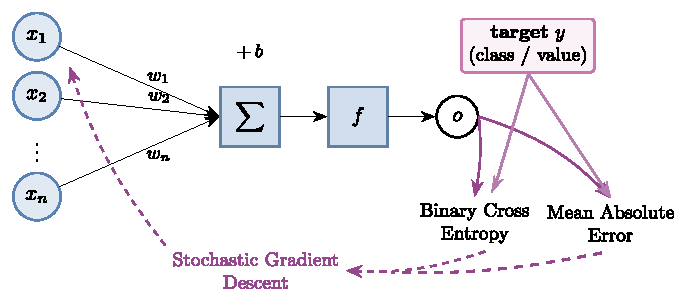
\includegraphics[width=0.85\textwidth]{ch02_sota/figures/perceptron.pdf}
    \caption{The Perceptron, the basic unit of a neural network. The
    inputs $x_1, \dots, x_n$ are weighted by $w_1, \dots, w_n$, summed
    together with a bias $b$, and passed through an activation function
    $f$ to produce the output $o$. During training, $o$ is compared to a
    target $y$ through a loss --- binary cross-entropy for classification,
    mean absolute (or squared) error for regression --- and the weights
    are updated by back-propagation and stochastic gradient descent.}
    \label{fig:perceptron}
\end{figure}

\textbf{The multi-layer perceptron} \citep{rumelhart1986learning} stacks many perceptron units into
layers and composing them yields a \acrshort{DNN}, but the learning
principle is already visible in a single unit. Training begins from \emph{randomly initialised} weights and proceeds by
making the output $o$ progressively closer to a target $y$ by a \emph{loss} $\mathcal{L}(o, y)$ whose form depends on the task. For a
\emph{classification} task the target $y$ is a class label and a common
choice is the binary cross-entropy, $\mathcal{L}_{\mathrm{BCE}}(o, y) = -\big[\, y \log o + (1-y)\log(1-o)\,\big] $, whereas for a \emph{regression} task --- the family this thesis focuses
on, where $y$ is itself a signal --- the loss measures a numerical
distance, such as the mean absolute error $ \mathcal{L}_{\mathrm{MAE}}(o, y) = \lvert o - y \rvert $. 

The weights are then adjusted to reduce this loss by
\emph{back-propagation}, which computes the gradient of the loss with
respect to every parameter, followed by \acrfull{SGD}, which takes a small
step against that gradient: $\theta \leftarrow \theta - \eta\, \nabla_\theta \mathcal{L}(o, y) $, where $\eta$ is the learning rate. Because evaluating the expectation in Equation~\ref{eq:erm} over the whole dataset at once is impractical, in
practice \acrshort{SGD} approximates it on small random subsets of the
data, the \emph{mini-batches}: each iteration of \acrshort{SGD} is
computed on a fresh mini-batch, and the loop is repeated until the loss
converges. This cycle --- forward pass, loss, back-propagation,
parameter update --- is the engine behind every model in this thesis. Crucially, all of the above presupposes that for every input $x$ we have
access to its corresponding target $y$: it is the pairing $(x, y)$ that
makes the loss in Equation~\ref{eq:erm} computable. This is
known as \emph{supervised learning}.

\textbf{The \acrfull{CNN}} \citep{lecun1998gradient} was a pivotal refinement: instead of learning an independent weight for every input--unit connection, we learn a set of
\emph{filters} (or \emph{kernels}) that are slid across the input, as
illustrated in Figure~\ref{fig:cnn}. Each is applied at
every spatial location, so the same weights are reused throughout the
input --- a form of weight sharing that drastically reduces the number of
parameters and builds in translation equivariance. \acrshort{CNN}s were
first popularised for handwritten-digit recognition and, more than a
decade later, became the workhorse of computer vision.


\begin{figure}[htbp]
    \centering
    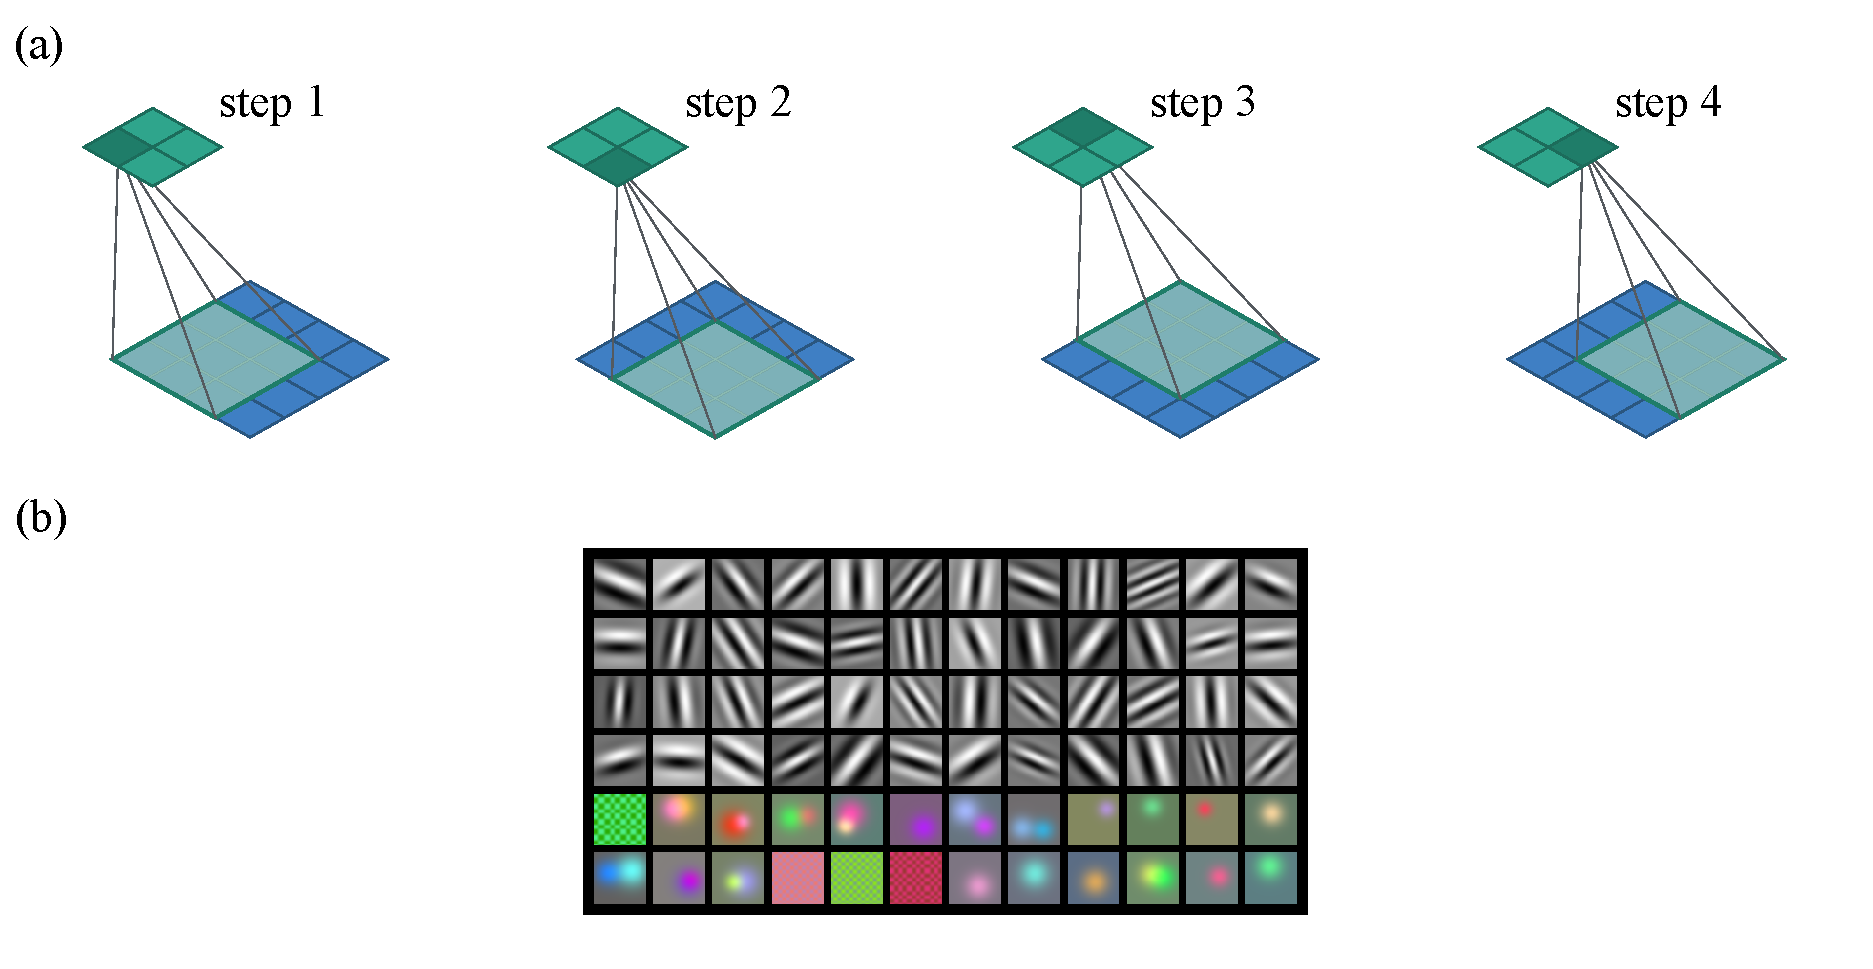
\includegraphics[width=0.9\textwidth]{ch02_sota/figures/cnn_kernel.pdf}
    \caption{Convolutional filters in a \acrshort{CNN}. \textbf{(a)}~A
    $3\times3$ filter (kernel) slid across a $4\times4$ input image or feature map (blue) to produce a $2\times2$ output feature map (green); at each of
    the four positions the filter covers a local region of the input
    (highlighted) and produces a single output value. \textbf{(b)}~Illustrative examples of filters learned: the grayscale filters (top) resemble oriented Gabor functions acting as edge detectors, while the colour
    filters (bottom) capture colour-opponent and low-frequency patterns.}
    \label{fig:cnn}
\end{figure}


In audio, the two-dimensional input is not an image but a
spatio-temporal representation of the signal, most commonly the
\acrfull{STFT}. Early systems operated on the magnitude spectrogram
alone, discarding the phase, although recent models process
the complex spectrogram \citep{tong2024scnet, schroter2022deepfilternet} --- real and imaginary parts jointly.

Sliding a filter over the input yields a smaller \emph{feature map}, one
per filter; stacking many filters per layer and many layers produces a
hierarchy of feature maps of increasing abstraction. While the
filters learned in the first layers of an image \acrshort{CNN} resemble
Gabor functions tuned to particularly oriented edge detectors
(Figure~\ref{fig:cnn}); in music, the analogous  filters
tend to specialise instead on timbre or rythm respectively. Deeper layers compose these primitives into progressively complex detectors
for more concrete concepts --- particular colours or shapes
in vision, or higher-level acoustic patterns in audio.

Formally, writing $\mathbf{H}^{(0)} = x$ for the input and $\ast$ for the
convolution, the $k$-th feature map of layer $l$ is
\begin{equation}
    \mathbf{H}^{(l)}_{k} = f\!\left(
        \sum_{c=1}^{C_{l-1}} \mathbf{W}^{(l)}_{k,c} \ast \mathbf{H}^{(l-1)}_{c}
        + b^{(l)}_{k} \right),
    \label{eq:conv}
\end{equation}
where the learned filters $\mathbf{W}^{(l)}_{k,c}$ and biases $b^{(l)}_{k}$
now play the role of the parameters $\theta$ of Equation~\ref{eq:erm}, and
$f$ is the (non-linear) activation, typically a rectified linear unit.
After $L$ such layers, interleaved with pooling operations that
progressively reduce the spatial resolution, the final feature maps are
flattened into a single vector $
    z = \mathrm{vec}\!\left(\mathbf{H}^{(L)}\right) \in \mathbb{R}^{d} $
known as the \emph{embedding}: a compact, learned representation of the
input that concentrates the information relevant to the task. The output
is then a simple --- often linear --- read-out of this embedding, $o = f_\theta(x) = g\!\left(\mathbf{W}_{o}\, z + \mathbf{b}_{o}\right)$
with $g$ a softmax over classes for a classification task. The embedding
is a central object in modern deep learning: because it distils the
task-relevant content of the input into a fixed-size vector, the same
embedding can often be reused for tasks other than the one it was trained
on --- an idea we return to when discussing pre-trained representations.

A canonical example is the VGG network
\citep{simonyan2014very}, sketched in Figure~\ref{fig:vgg16}: a deep stack
of small $3\times3$ convolutions and max-pooling layers that successively
halve the spatial resolution while increasing the number of feature maps,
followed by a few fully connected layers that map the final embedding to
the output classes.

\begin{figure}[htbp]
    \centering
    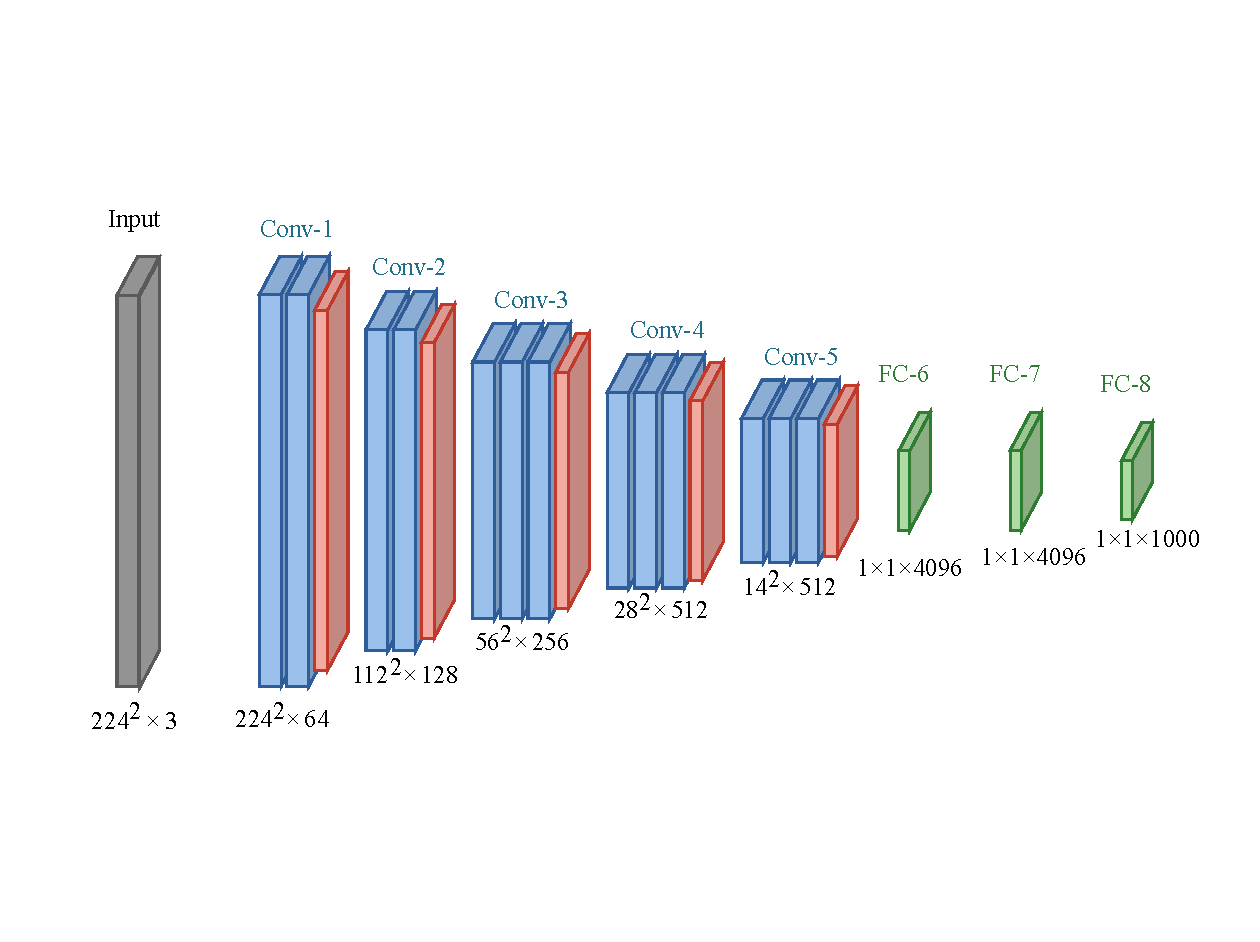
\includegraphics[width=.8\textwidth, trim={.25cm 3cm .25cm 1.3cm}]{ch02_sota/figures/vgg16.pdf}
    \caption{The VGG-16 architecture \citep{simonyan2014very}, a canonical
    \acrshort{CNN}. Stacks of $3\times3$ convolutions (blue) followed by
    max-pooling (red) progressively reduce the spatial resolution while
    increasing the number of feature maps, until a small set of fully
    connected layers (green) maps the final embedding to the $1000$ output
    classes.}
    \label{fig:vgg16}
\end{figure}


Beyond a certain depth, adding more layers
makes the network harder to optimise. ResNets \citep{he2016deep}
resolved this with a simple architectural change. Rather than asking a
stack of layers to fit a target mapping $\mathcal{H}(x)$ directly, a
ResNet lets it fit only the \emph{residual}
$\mathcal{F}(x) = \mathcal{H}(x) - x$ and adds the input back through an
identity \emph{skip} connection, so that the block computes
$\mathcal{F}(x) + x$ (Figure~\ref{fig:resnet}). The intuition is
that if the optimal mapping is close to the identity --- as it often is
for the incremental refinements performed by successive deep layers ---
it is far easier to drive $\mathcal{F}(x)$ towards zero than to fit the
identity with a stack of non-linear layers.
 
Visualisations in \citet{li2018visualizing} show that skip connections
dramatically smooth the $\mathcal{L}$ loss landscape: the rugged, highly
non-convex surface of a deep plain network gives way to a far smoother, near-convex one that gradient descent can navigate much more easily (Figure~\ref{fig:resnet}). 

\begin{figure}[hb]
    \centering
    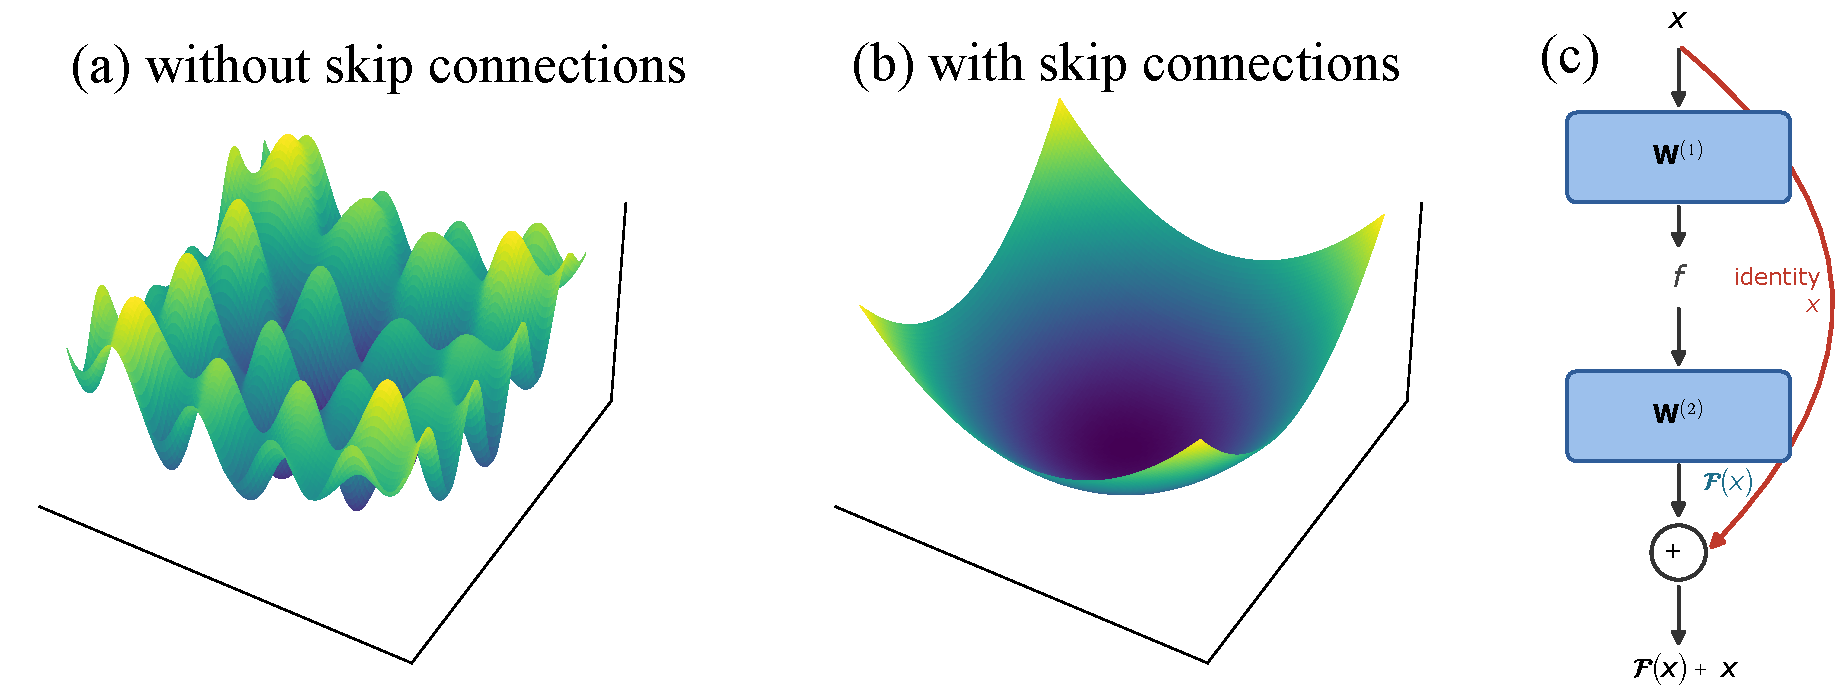
\includegraphics[width=.9\textwidth]{ch02_sota/figures/resnet.pdf}
    \caption{Residual networks. Effect of skip connections on the loss landscape (illustrative):  \textbf{(a)}~a deep plain network exhibits a rugged  highly
    non-convex $\mathcal{L}$ surface with many poor local minima, whereas \textbf{(b)}~the
    same network with skip connections has a near-convex
    landscape much easier to optimise, following the
    visualisation of \citet{li2018visualizing}.      
    \textbf{(c)}~A ResNet block: the two
    weight layers $\mathbf{W}^{(1)}$ and $\mathbf{W}^{(2)}$, with activation
    $f$, map the input through the feature maps $\mathbf{H}_1$ and
    $\mathbf{H}_2 = \mathcal{F}(x)$ (the residual), and an identity skip
    connection (red) adds the input back, so the block outputs
    $\mathcal{F}(x)+x$.}
    \label{fig:resnet}
\end{figure}

Combining the two preceding ideas yields one of the most widely used
architectures in audio processing. Taking a VGG-like stack of convolutions
and pooling as a \emph{contracting} path that compresses the input into a
low-resolution, high-channel representation, and mirroring it with a
symmetric \emph{expanding} path that upsamples back to the original
resolution, gives an \emph{encoder--decoder}. Adding skip connections in
the spirit of ResNet --- here linking each encoder layer to the decoder
layer of matching resolution, so that fine-grained detail can bypass the
bottleneck and reach the output directly --- gives the U-Net
\citep{ronneberger2015u}. Originally proposed for image segmentation, it
has become the backbone of countless source-separation and
speech-enhancement models.

\begin{figure}[htbp]
    \centering
    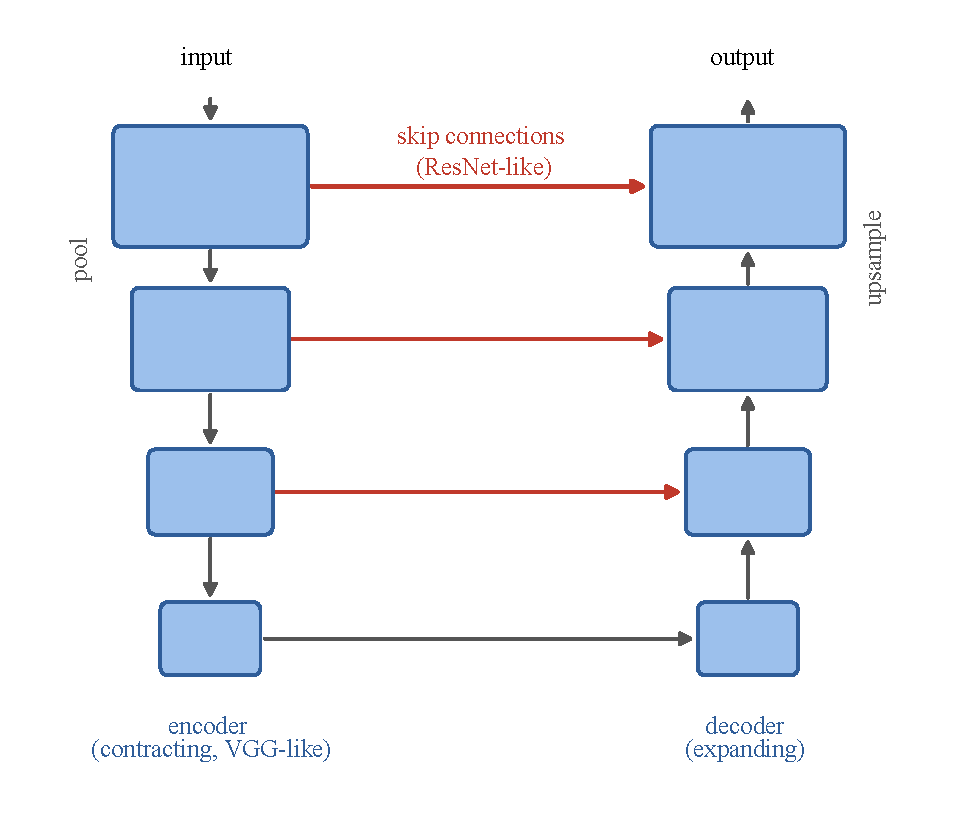
\includegraphics[width=0.72\textwidth]{ch02_sota/figures/unet.pdf}
    \caption{The U-Net as a combination of the two preceding models: a
    VGG-like encoder--decoder (blue) with ResNet-style skip connections (red). Details are omitted for clarity.}
    \label{fig:unet}
\end{figure}


\section{Spatial Audio and Ambisonics}
\label{sec:bg_spatial}
i aquí una subsecció.fdsaf

\section{Room Impulse Response simulation}
\label{sec:bg_rir}
i aquí una subsecció.fdsaf

\section{Task-specific scientific background}
\label{sec:tasks}
i aquí una subsecció.fdsaf

\subsection{Hearing Aids}
\label{ssec:bg_ha}
i aquí una subsecció.fdsaf

\subsection{Speech Enhancement}
\label{ssec:bg_se}
i aquí una subsecció.fdsaf

\subsection{Music Source Separation}
\label{ssec:bg_mss}
i aquí una subsecció.fdsaf